%%%%%%%%%%%%%%%%%%%%%%%%%%%%%%%%%%%%%%%%%
% Journal Article
% LaTeX Template
% Version 1.3 (9/9/13)
%
% This template has been downloaded from:
% http://www.LaTeXTemplates.com
%
% Original author:
% Frits Wenneker (http://www.howtotex.com)
%
% License:
% CC BY-NC-SA 3.0 (http://creativecommons.org/licenses/by-nc-sa/3.0/)
%
%%%%%%%%%%%%%%%%%%%%%%%%%%%%%%%%%%%%%%%%%

%----------------------------------------------------------------------------------------
%	PACKAGES AND OTHER DOCUMENT CONFIGURATIONS
%----------------------------------------------------------------------------------------

\documentclass[twoside]{article}
\usepackage{graphics, graphicx}
\usepackage{lipsum} % Package to generate dummy text throughout this template
\usepackage[sc]{mathpazo} % Use the Palatino font
\usepackage[T1]{fontenc} % Use 8-bit encoding that has 256 glyphs
\linespread{1.05} % Line spacing - Palatino needs more space between lines
\usepackage{microtype} % Slightly tweak font spacing for aesthetics

\usepackage[hmarginratio=1:1,top=32mm,columnsep=20pt]{geometry} % Document margins
\usepackage{multicol} % Used for the two-column layout of the document
\usepackage[hang, small,labelfont=bf,up,textfont=it,up]{caption} % Custom captions under/above floats in tables or figures
\usepackage{booktabs} % Horizontal rules in tables
\usepackage{float} % Required for tables and figures in the multi-column environment - they need to be placed in specific locations with the [H] (e.g. \begin{table}[H])
\usepackage{hyperref} % For hyperlinks in the PDF


\bibliographystyle{plainnat}
\usepackage{natbib}
\usepackage{lettrine} % The lettrine is the first enlarged letter at the beginning of the text
\usepackage{paralist} % Used for the compactitem environment which makes bullet points with less space between them
\usepackage{subcaption}
\usepackage{abstract} % Allows abstract customization
\renewcommand{\abstractnamefont}{\normalfont\bfseries} % Set the "Abstract" text to bold
\renewcommand{\abstracttextfont}{\normalfont\small\itshape} % Set the abstract itself to small italic text

\usepackage{titlesec} % Allows customization of titles
\renewcommand\thesection{\Roman{section}} % Roman numerals for the sections
\renewcommand\thesubsection{\Roman{subsection}} % Roman numerals for subsections
\titleformat{\section}[block]{\large\scshape\centering}{\thesection.}{1em}{} % Change the look of the section titles
\titleformat{\subsection}[block]{\large}{\thesubsection.}{1em}{} % Change the look of the section titles

\usepackage{fancyhdr} % Headers and footers
\pagestyle{fancy} % All pages have headers and footers
\fancyhead{} % Blank out the default header
\fancyfoot{} % Blank out the default footer
\fancyfoot[RO,LE]{\thepage} % Custom footer text

%----------------------------------------------------------------------------------------
%	TITLE SECTION
%----------------------------------------------------------------------------------------

\title{\vspace{-15mm}\fontsize{24pt}{10pt}\selectfont\textbf{Finding Grammatical Structure}} % Article title


\author{
\large
\textsc{David Rau (11725148), Jer\^ome Mutgeert (....)},Maartje de Jonge (.....) \\[2mm] % Your name
\normalsize University of Amsterdam \\ % Your institution
\normalsize \href{mailto:david.rau@student.uva.nl, ...,...}{david.rau@student.uva.nl, ..., ...} % Your email address
\vspace{-5mm}
}
\date{}


%----------------------------------------------------------------------------------------

\begin{document}

\maketitle % Insert title

\thispagestyle{fancy} % All pages have headers and footers

%----------------------------------------------------------------------------------------
%	ABSTRACT
%----------------------------------------------------------------------------------------

\begin{abstract}

\noindent 
- main idea
- key findings

\end{abstract}

%----------------------------------------------------------------------------------------
%	INTRODUCTION
%----------------------------------------------------------------------------------------

\begin{multicols}{2} % Two-column layout throughout the main article text

\section{Introduction}
- motivation

- problem area

- problem itself

- research question

- approach

\paragraph{Outline}
The remainder of this report is organized as follows \ldots


%----------------------------------------------------------------------------------------
%	BACKGROUND
%----------------------------------------------------------------------------------------

\section{Background}
\label{background}

- what is language modeling?

- what kind of language modelling did we study?

- what is the problem that we focus on?


%----------------------------------------------------------------------------------------
%	PREVIOUS WORK
%----------------------------------------------------------------------------------------

\section{Related Work}
\label{related work}

%summary of ~\citep{Linzen2016}

%Linzen 2016

%%%% Research Question
LSTM
- can capture long distance statistical regularities
- do not explicitly incorporate syntactic structure
- question: can LSTM capture dependencies that follow from syntactic structure, from a corpus without syntactic annotations?
- more specific: investigate number agreement in English subject-verb dependencies
as an example of a structure sensitive dependency

%%%% Experiments
- train models with different training objectives
  - with explicit grammatical target as training objective
    - number prediction
    - verb infliction
    - grammatical judgement
  - a more generic language model with the objective to predict the next word
- corpus: wikipedia

- evaluate how these models perform on simple and more complex sentences:
  - simple cases: noun that is the subject closeby verb, no intervening nouns
  - effect of long distance: lot of words inbetween noun and verb
  - complex cases: intervening nouns with different number inbetween head of subject noun and verb
  
%%%% Results
- high or reasonable overall accuracy for all models, explained by the fact that most real world sentences are actually simple (no attractors)
   - NP, VI, GJ, LM
- all explicitly trained language models perform reasonable on complex cases.
   - distance
   - attractors
- language model performs bad on complex cases. sensitive to most recent noun.
  - more complex objective, lack of data? no, google also fails.

%%%% Detailed analysis of results
More detailed error analysis shows that
- function words are important, by comparing with a baseline model trained on noun verb sequences
- relative clauses are challenging, especially when relativizer misses
- some errors in identifying nouns (due to ambiguity: drives) and identifying the number of a noun

- activations: units that track main subject, subject of current clause, embedding status, number of main clause subject/most recent noun

%%%% Conclusion
- LSTM can capture grammatical structure given targeted supervision
- language modeling is insufficient for capturing syntax sensitive dependencies
- authors advice: supplement language modeling objectives with more explicit targets
for tasks in which it is desirable to capture syntactic dependencies.


\section{Problem Analysis}
\label{problem}

- How does the language model decide between plural or singular form in sentences like ``The products that the company [produce/produces]'' or ``The products of the company [are/is]''?

- The model needs to decide the dependency relations between verbs and nouns,
and it has to decide the count of nouns and verbs.
We assume that the model is able to `learn' the count of a noun or verb (may fail for some nouns as discussed in Linzen). We focus this discussion on how the model may infer dependencies. 

- syntactic clues. Example: the word `that' indicates the beginning of a relative clause with a noun and a verb, therefore the noun 'companies' is associated with the verb `produce' in the first sentence. In contrast, the word `of' in the second sentence indicates a possessive relation with a noun and does not expect a verb, therefore the noun company is not associated to the verb `are' in the second sentence.

- semantic clues. Example: the noun 'companies' is associated with the verb 'produce' in the first sentence because this combination of words (company/companies ... produces/produce) appears a lot in the training sentences
\\
\textit{Hypothesis: the model uses both semantic and syntactic clues to determine which
form of the verb is most likely (singular/plural).
}
\\
EXPERIMENT IDEA 1:
We investigate whether the model (primarily) uses semantic or syntactic clues to determine the singular/plural form of the verb. 
We do this by

1. observing how the model behaves on sentences in which semantic and syntactic clues are consistent with each other, e.g. ``The products that the company [produce/produces]''

2. observing how the model behaves on sentences that are semantically nonsense, e.g. ``The products that the company [swim/swims]''

3. observing how the model behaves on sentences in which semantic and syntactic clues contradict each other, e.g. ``The companies that the product [produce/produces]''. 

We generate these sentences using nouns and verbs that occur frequently in the corpus (lots of semantic info) and for nouns and verbs that occur 
infrequently (not so much semantic info). We compare the results of all six combinations.

EXPERIMENT IDEA 2:
(future work?) A different but related question is whether
syntax (function words) alone provides enough information 
to decide the plurality of verbs.
We investigate this question (for the english language). 
First we 'strip the semantic clues' from the sentences by replacing all nouns and verbs with their pos tag, e.g ``The NNS that the NN [VBP/VBZ]''. Then we perform two experiments: 
2a) we ask humans to decide the plurality of the verbs for a set of test sentences
in this form. Can humans decide the plurality of a verb without knowing the meaning of the verb and the nouns?
2b) we train a model on these kind of processed sentences with the target
to decide the plurality of the verb.
We then ask the model to complete the sentences of a test set in the stripped form. 
Can the model learn to decide the plurality without knowing the meaning of
the verb and the nouns?


%----------------------------------------------------------------------------------------
%	EXPERIMENTS
%----------------------------------------------------------------------------------------

\section{Experiments}
\label{experiments}

\textbf{Data:} 
The language model was tested on lower case sentences that were generated from the Wall Street Journal section of the Penn Treebank \citep{Marcus1993}. Therefore, 40 nouns and verbs, that were amongst the most common and occur in the test corpus as well as in language model's corpus, were extracted. Those words build the base for the sentence generation for the subsequent experiments. 

\textbf{Model evaluation:} In order to evaluate the performance of our model, we query it with the sentence containing both, the plural (\ref{sent:wrong}) and the singular (\ref{sent:right}) mode of the verb: 

\begin{equation}
	\label{sent:wrong}
	\textnormal{the producer plan}
\end{equation}
\begin{equation}
	\label{sent:right}
	\textnormal{the producer  \textbf{plans}}
\end{equation}




The model provides probabilities for both sentences. We choose the sentence with the higher probability and compare whether it matches the correct solution (\ref{sent:right}).

\subsection{Replication Linzen 2016}
\label{replication}
According to the experiments in \citep{Linzen2016} we examine the models error rate predicting the number of a verb in a sentence when nouns intervene between the subject and the verb. 

We next test how the model's ability to predict the number of the verb is affected by none and one intervening noun, respectively. If there is an intervening noun we keep track whether the number of the noun differs from the number of the subject. In this way we can easily spot whether the model makes use of the most obvious heuristic: choosing the the number of the verb only in dependence of the last attractor in the sentence.

As depicted in Figure \ref{fig:2b} our model performs slightly better for plural subjects (18.7\% error rate) than for singular (14,1\% error rate) when no attractors are present in the sentence. An intervening noun with the same number as the subject causes a decrease of the error rate to 18.1\% and 13.3\%, respectively. Surprisingly, when the number of the subject differs from the intervening noun the error rates increased dramatically; in singular subjects to 62,3\% in plural subjects to 59,0\%.

In the following we examine the error rate when adding multiple attractors to the sentence. In order to avoid the model of being distracted by an intervening noun with same number as the subject we only insert nouns with the same number . \citep{Linzen2016} refer to such as  \textit{ dependencies with homogeneous intervention}. In (\ref{sent:right2}) the underlined represent homogeneous interventions, whereas in (\ref{sent:wrong2}) the number of the nouns differ. The bold words highlight the dependency between noun and corresponding verb.

\begin{equation}
	\label{sent:right2}
	\textnormal{the \textbf{interest} in the \underline{shares} of the \underline{businesses} \textbf{rises} \dots}
\end{equation}
\begin{equation}
	\label{sent:wrong2}
	\textnormal{the \textbf{interest} in the \underline{shares} of the \textit{business} \textbf{rises} \dots}
\end{equation}
Figure \ref{fig:2c} shows that with an increasing number of noun interventions the error rate goes from 18.2\% (0 attractors) up to 49.6\% (4 attractors) which is close to randomly guessing the number of the verb. 
\end{multicols}

\begin{figure}
    \centering
    \begin{subfigure}[b]{0.4\textwidth}
    \caption{}
        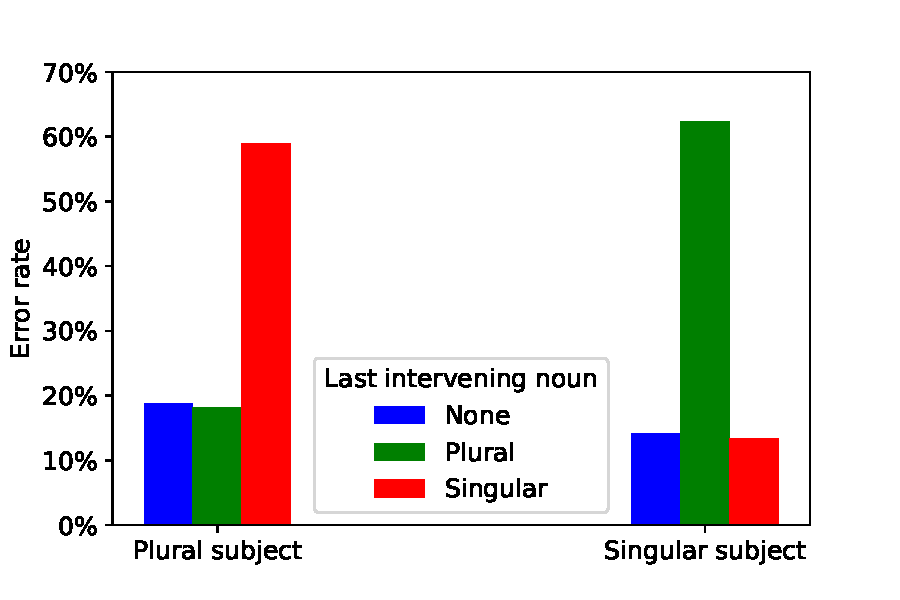
\includegraphics[width=\textwidth]{2b.pdf}
        \label{fig:2b}
    \end{subfigure}
    ~ %add desired spacing between images, e. g. ~, \quad, \qquad, \hfill etc. 
      %(or a blank line to force the subfigure onto a new line)
    \begin{subfigure}[b]{0.4\textwidth}
    	\caption{}
        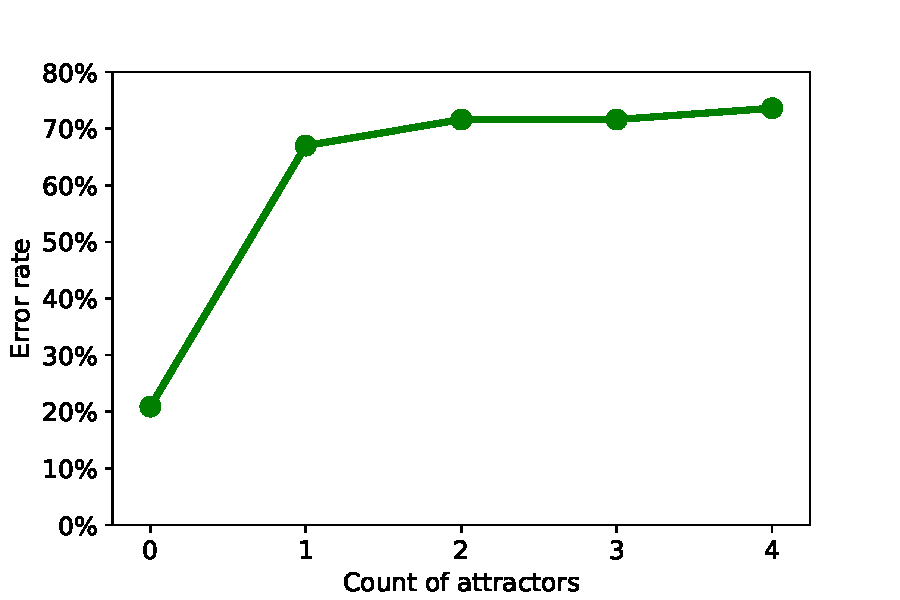
\includegraphics[width=\textwidth]{2c.pdf}
        \label{fig:2c}
    \end{subfigure}
    \caption{Error rates of the language model plotted against: \ref{fig:2b} presence and number of last attractor; \ref{fig:2c} count of attractors in dependencies with homogeneous intervention}
\end{figure}

\begin{multicols}{2}



\subsection{Own Experiments}
\label{own-experiments}

- We investigate the following question about grammatical structure \ldots

%----------------------------------------------------------------------------------------
%	CONCLUSION
%----------------------------------------------------------------------------------------
\section{Conclusion}
\label{conclusion}

- Conclusion \ldots

%----------------------------------------------------------------------------------------
%	DISCUSSION
%----------------------------------------------------------------------------------------
\section{Discussion}



%----------------------------------------------------------------------------------------
%	REFERENCE LIST
%----------------------------------------------------------------------------------------

\bibliographystyle{abbrv}
\bibliography{article}


%----------------------------------------------------------------------------------------

\end{multicols}

\end{document}
